\chapter{Introduction}
\label{chap:scaling_introduction}

\begin{flushright}{\slshape    
The allometric law promises to become\\
an integral part of geography theory.} \\ \medskip
--- David Harvey (1969)~\cite{Harvey:1969} 
\end{flushright}


\section{Probing cities with scaling laws}
\label{sec:probing_cities_with_scaling_laws}

\subsection{Scaling laws}
\label{sub:scaling_laws}

As discussed in the introduction of this thesis
(Chapter~\ref{chap:studying_cities}), cities are paradigmatic examples of
complex systems. As systems, they can be of thought of as `black boxes'
with inputs (people, goods, money, information, etc.), a structure (roads,
buildings, electric cables, etc.) and outputs (Patents, $CO_2$ emissions, etc.).

A simple way to explore the behaviour of such a system is to look at the way it
 behaves when we change its size. That is, how its structure and its
outputs change when the inputs are altered. Formally speaking, we try to find
the function $f$ such that the quantity $Y$ -- a measure of the output or the
structure -- varies as

\begin{equation}
    Y = f(S)
    \label{eq:functional_form}
\end{equation}

where $S$ is the size of the system. What is to be considered as the size of the
city? The answer, adopted by many before this thesis~\cite{Stewart:1947,
Bettencourt:2007}, is the total number of inhabitants. 

Why population, when the spatial footprint, the total volume occupied by its
building also seem like reasonable quantities? The honest reason is probably
purely a a pragmatic one: ``it works''. The afterthought, is that cities are
more than roads and buildings: cities are the people who inhabit them. People
are responsible for the changes in wealth, employment, number of patents. People
need new roads, and it is people who build them. People need electricity, and
again it is people who run electric cables between buildings. Inhabitants in a
city are the elements that interact constantly, and in their actions and
interactions are reponsible for the collective mechanisms that act on a larger
scale on the city as a whole.  In a sense, in the use of the population $P$ to
measure the size of a city as a system hides the understanding that cities are
the people that inhabit them.\\

Functional forms like the one presented in Eq.~\ref{eq:functional_form} with the
population $P$ used as a proxy for the size of the city turn out to be 
\emph{allometric scaling relationships}.

Allometric scaling relationships present themselves in the form of a power-law
relationship between various quantities $Y$ and the population size $P$ of
cities \emph{in a given system of cities} 

\begin{equation}
    Y = Y_0\,P^{\,\beta}
    \label{eq:scaling_definition}
\end{equation}

where the exponent $\beta$ can be different from $1$. This type of scaling
relation, used extensively in Biology~\cite{Thompson:1942} and in
Physics~\cite{Barenblatt:1996}, is a signature of the various processes
governing the phenomenon under study, especially when the exponent $\beta$ is
different from what would be naively expected. 

Three qualitatively different regimes are usually distinguished for the exponent
$\beta$~\cite{Bettencourt:2007}

\begin{description}
    \item[Superlinear] when $\beta>1$. In this situation, the $Y$ per capita
        increases with population size. This is associated with the notion of
        increasing returns with scale in economics.
    \item[Linear] when $\beta=1$. In this situation, the $Y$ per capita is
        constant. This behaviour is characteristic of an extensive system, when
        the whole is nothing but the sum of its parts.
    \item[Sublinear] when $\beta<1$. In this situation, the $Y$ per capita
        decreases with population size. When $Y$ is the cost in infrastructure,
        this is characteristic of economies of scale.
\end{description}    

\begin{figure}[!h]
    \centering
    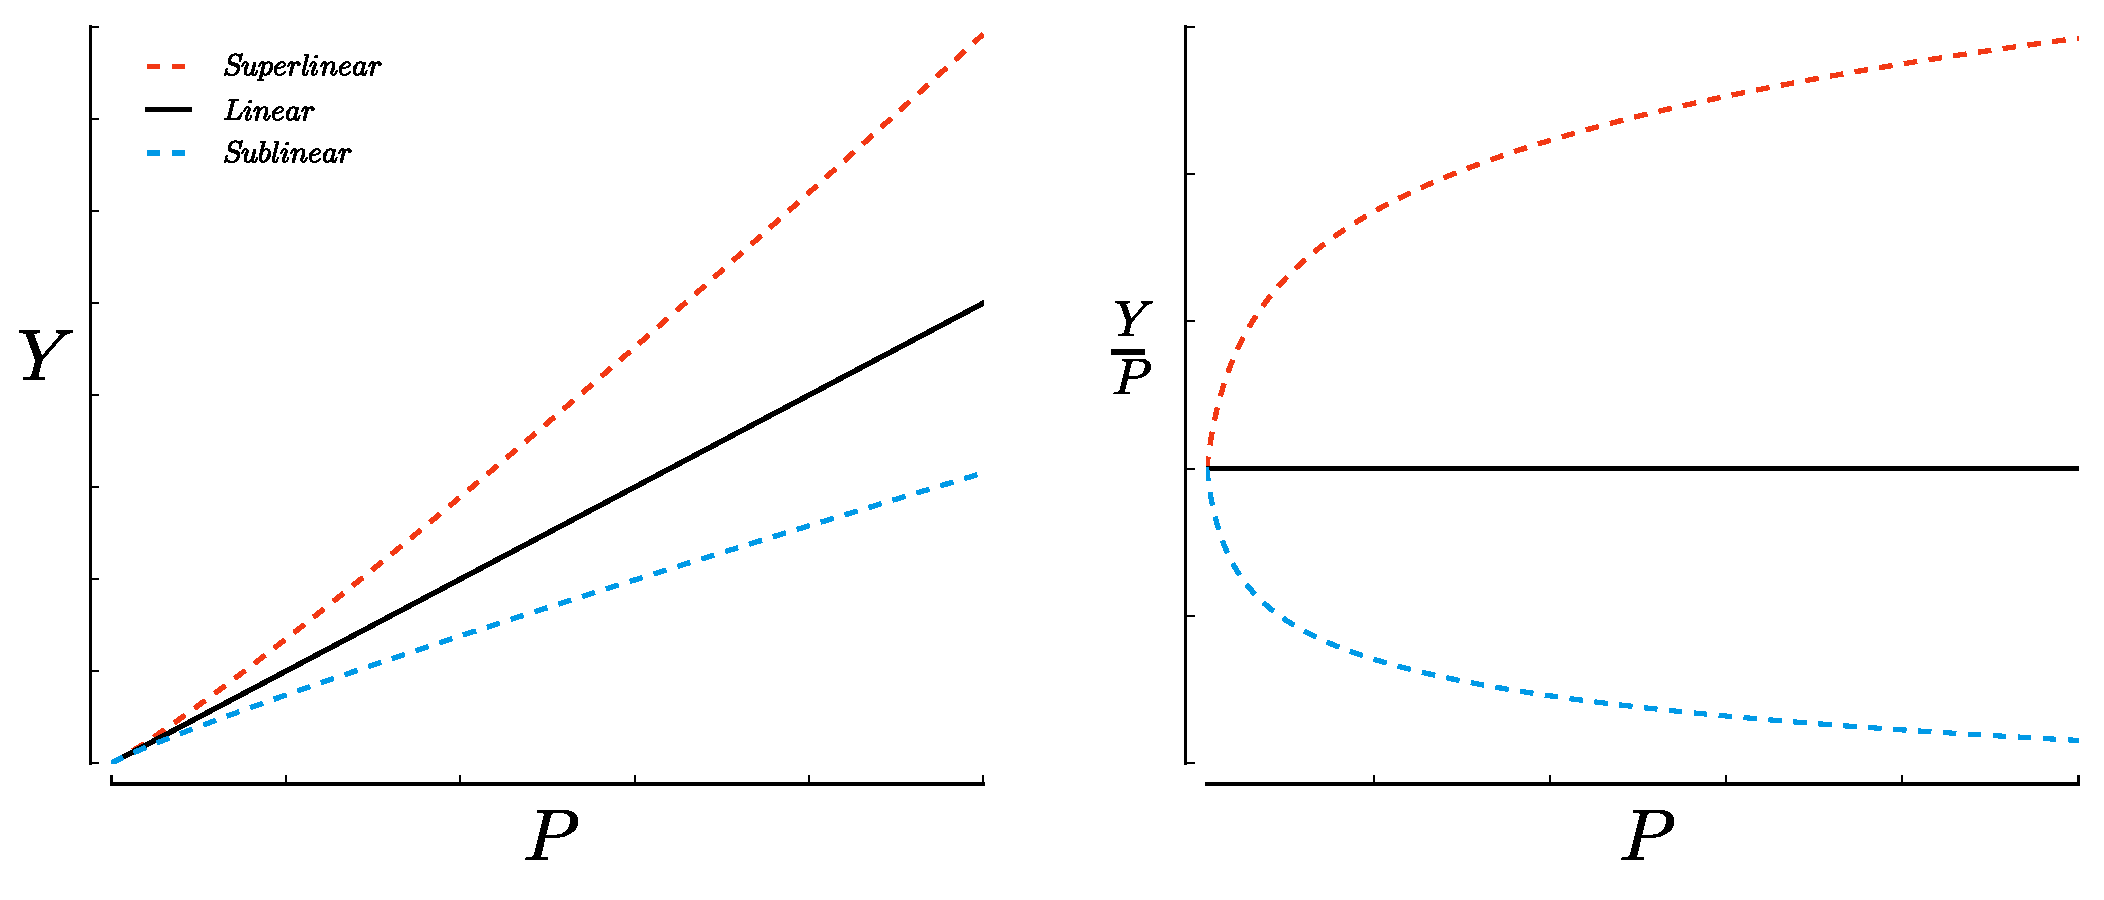
\includegraphics[width=\textwidth]{gfx/chapter-scaling/scaling_scheme.pdf}
    \caption{{\bf Sublinear, Linear and Superlinear scaling.} (Left) Example of a linear (black), sublinear (blue) and superlinear (red)
    behaviour. (Right) Evolution of the correspondant per-capita quantities with
population. A superlinear behaviour means that per-capita quantity increase with
population size, while a sublinear behaviour means per-capita quantities
decrease with city size.\label{fig:scaling_scheme}}
\end{figure}


We note that the scaling exponent $\beta$ is also directely related to the \emph{elasticity}
defined in Economics. Indeed, the cities' population elasticity of the quantity
$Y$ is defined as\\

\begin{equation}
    \beta = \frac{dY/Y}{dP/P}
\end{equation}


\subsection{Underlying assumptions}
\label{sub:underlying_asumptions}


Several assumptions, although rarely mentionned, hide behind every exhibited
scaling law relationships.

The first one, is that we are able to unambigusouly delineate cities as systems.
While this is trivial in the case of animals (it is fairly easy for us to
isolate an elephant, or a cat from its environment to measure its mass and its
metabolic rate), it is a much more difficult task in the case of cities.
Indeed, cities do not have fixed boundaries, the geographical limits of the
object studied evolves with time, as people are born and die, change residence
and as companies do the same.  Traditionnally, people have relied on the
definition given by statistical agencies of the respective countries they were
studying -- and we will do the same in the next chapter. We will however see, in
the chapter concluding this part, that the problem of delineating cities is a
sensible issue and affects greatly scaling analyses. \\


A second issue, rarely -- if ever -- mentionned in the literature, is the
necessity to define the set of cities to study. Scaling laws are essentially
cross-sectional relationships, where we measure the quantity $Y$ on a set of
cities with different populations. But is the set determined? For instance,
would it make sense to mix French cities, Ukrainian, Canadian and Korean, etc
cities and plot, say, their total GDP as a function of the population? Would we
then observe a neat scaling relationship? 

Intuitively, this is very unlikely to happen, as different countries have
overall different levels of wealth, and this should be reflected in the wealth
of their cities. Therefore, plotting cities from different countries together is
likely to introduce important deviations to the pure scaling relations which are
not due to the fact that cities in different countries do not follow the same
processes, but rather because of systemic differences at the country level. As a
matter of fact, most studies limit themselves to a single country. One should
bear in mind tha this choice is arbitrary, however. And the problem of chosing
the appropriate set from which to pick the cities is linked to the more general
problem of defining systems of cites.


\subsection{An increasing importance in the urban landscape}
\label{sub:an_increasing_place_in_the_landscape}


The epigraph used at the beginning of this chapter, found in Harvey's 1969
\emph{Explanation in Geography}, is somewhat prophetic.  Allometric scaling
relationships only concern $1$ page out of the $500$ pages that the book
contains, a reflection of the very few empirical results that were available at
the time.  Looking at the extent of the literature on scaling relationships
almost $50$ years after Harvey wrote this sentence, it is difficult to deny the
accuracy of this prophecy. Thanks to the wider availability of data through
statistical agencies, but also the availability of 'new data' (such as mobile
phone data), empirical measurements of scaling laws have multiplied, and now
concern quantities as diverse as the total surface area, the number of patents,
the quantity of $CO_2$, the number of phone contacts of individuals, etc. 
The discovery of allometric scaling in cities is not recent~\cite{Stewart:1947},
but it has undoubtedly caused a stir in the literature about urban systems over
the last
decade~\cite{Bettencourt:2007,Pumain:2004,Bettencourt:2013,Louf:2014_scaling,Louf:2014_smog,Arcaute:2014}.\\


In the next section, we will present a non exhaustive historical review of the
empirical results on scaling relationships. I will then discuss the existing
theoretical frameworks. This will lay the ground for our contribution to the
debate: a theoretical interpretation of the scalings related to the mobility of
people, and an estimate for the scaling exponent of the surface area.  



\section{A brief history of allometric scaling and cities}
\label{sec:a_brief_history_of_allometric_scaling_and_cities} 

Rather than an exposition that is linear in time, we deliberately chose to
classify the proposed studies according to studied quantity in order to
emphasize the variety of variables that have been studied. Incidentally, this
order also reveals the different waves of interest scaling relationships have
sparked off in the past $6$ decades. 

\subsection{Surface area}
\label{sub:surface_area}

The spatial footprint of cities, as can be observed on satellite picture or on
maps, is one of the properties that is easiest to measure. It is therefore not
surprising that the first occurence of the scaling relationships in cities was
the scaling of the surface area of cities with their population. In $1947$,
using data about administrative cities obtained from the $1940$ US Census, John
Stewart shows
\graffito{Incidentally, the author of the study, John Stewart, was a physicist.}

\begin{equation}
    A = \frac{P^{\,3/4}}{350}
\end{equation}

The next occurence of this scaling can be found $9$ years later in a study by
the same author~\cite{Stewart:1958}, using UK census data. From there, it isn't
long until the result percolates in Geography with Boyce in $1963$~\cite{Boyce:1963}.
In $1965$, Nordbeck's paper~\cite{Nordbeck:1965} also studies the scaling of surface area
with population, and, for the first time, explicitly refers to allometry in
biology. Later, Tobler~\cite{Tobler:1969} uses some of the first available
satellite images to provide the first confirmation using satellite pictures.
Satellite pictures were also used more recently by Gu\'erois in~\cite{Guerois:2003}.\\

When applied to morphological definitions of cities, all studies
(see~\cite{Batty:2011}) give an exponent that varies in the range $[0.70,
0.90]$. However, different results are obtained for functional definitions of
cities~\cite{Batty:2011}, or when the set of studied cities span several systems of
cities~\cite{Fuller:2009}.

Thus, despite being the oldest and most trusted scaling relationship in the
literature, the relation between the surface area and population size of cities
exhibits some of the issues we will discuss in
Chapter~\ref{chap:scaling_implication}.



\subsection{Economic diversity and employment}
\label{sub:economic_diversity}

\subsubsection{Employment diversity}
\label{ssub:employment_diversity}

The economic diversity has been of interest to researchers very early on. In
1949, Zipf in \emph{Human behavior and the principle of least
effort}~\cite{Zipf:1949} plots the number of service-business establishments, manufactures and
retail stores per city as a function of population (in log-log scale) using data
from the $1940$ US Census. He finds a linear relationship with population for
the three types of establishments, which agreed at the time with his model. He
also plots the scaling of the diversity, defined as the number of different kinds of
entreprises present in the city being studied. 

In his $1967$ \emph{Geography of market centers and retail
distribution}~\cite{Berry:1967} Berry, hoping to demonstrate the hierarchical
organisation of central places, plots this time the population of cities as a
function of the number of kinds of retail and service businesses observed.
Strangely enough, the data imply

\begin{equation}
    D \propto P^{\, \beta}
\end{equation}

with $\beta > 1$, in contradiction with later results found by Bettencourt et
al.~\cite{Bettencourt:2014}.\\

Indeed, Bettencourt et al.\cite{Bettencourt:2014} showed that the professional
diversity $D$, measured as the number of professions of different kind in the
city considered, could be fitted by the following function

\begin{equation}
    D(N_e) = d_0\, \frac{\left(\frac{N_e}{N_0}\right)^\gamma}{1+\left(\frac{N_e}{N_0}\right)^\gamma}
\end{equation}

where $d_0$ is the size of the classification used in the data, $N_0$ is the
typical saturation size, and $\gamma < 1$ is an exponent expressing the extent to
which new activities `appear' as the total employment increases. 

\subsubsection{Employment in different activities}
\label{ssub:employment_in_different_activities}

More recently, Pumain and coauthors~\cite{Pumain:2006}, extending the work done
by Paulus in his PhD thesis~\cite{Paulus:2004}, showed that the
employment in different activities in cities scaled as

\begin{equation}
    E_a \propto P^{\,\beta}
\end{equation}

with different exponents $\beta$ for the different activities. They observed,
for the year $1999$ in France, that the exponents could be classified in three
categories

\begin{itemize}
    \item $\beta > 1$ for innovative sectors: research and developpement,
        consultancy.
    \item $\beta = 1$ for common sectors: hotels, health and social services,
        education.
    \item $\beta < 1$ for `mature' sectors such as the food industry
\end{itemize}

This result was confirmed recently by Youn et al.~\cite{Youn:2014} (although
they do not refer to this previous work), who showed that the same behaviour was
observed for the number of business of a given type. A particularly interesting
result shown by Pumain et al.~\cite{Pumain:2006} is the evolution of the
different exponents with time, where we can see a clear increase of the
exponents for research and developpement, and a clear decrease of the exponents
related to manufactures of different kinds. This behaviour in time is the
starting point of the authors' evolutionary theory to explain scaling laws, that
we will discuss later in this introduction.\\


\subsection{Wealth}
\label{sub:wealth}

Although the notion of increasing returns with the size of the agglomeration is
often discussed in economics, although emprical proofs are hard to find. The
superlinear scaling of the GDP of american cities as a function of their
population may be the most striking example of such increasing
returns~\cite{Bettencourt:2007}. In the same article, Bettencourt et al. showed
that the number of patents (used as a proxy for creativity) also scaled
superlinearly with population size in the US.

Because larger cities create proportionally more wealth than smaller cities, we
can wonder whether this supplement of wealth allows to sustain proportionally
more jobs. The answer, as shown in~\cite{Bettencourt:2014} for american cities,
is negative: the total employment of a city is on average proportional to its population.

\subsection{Human interactions}
\label{sub:human_interactions}

At the heart of Bettencourt's model~\cite{Bettencourt:2013} to explain the
superlinear scaling of quantities associated with wealth and creativity is the
behaviour of the total number of interactions between individuals with the size
of the city. In an attempt to test this hypothesis, Schl\"apfer et
al.~\cite{Schlapfer:2014} looked at the scaling of the cumulative number of
contacts $K$ that people had over the phone, using mobile phone data in
Portugal, and landlines in the UK. They also looked at the cumulative call
volume (total number of minutes called) and the cumulative number of calls, and
found that the three quantities scale superlinearly with population size. 

They further found that the number of non-returned calls showed a larger
exponents than the number of calls, meaning that the number of solicitations an
individual gets is greater in large cities.\\

Although this is not emphasized by the authors of the study, we note that the
exponents found in Portugal vary with the city definition that is chosen, with a
clear superlinear behaviour for Portugal's municipalities and `statistical
cities', but a near-linear behaviour for LUZ (Larger Urban Zones, a functionnal
definition of cities introduced by Eurostat).


\subsection{Mobility of individuals, and environmental impact}
\label{sub:mobility}

Because cars are widely used (at least in the U.S.), and because peak travel
demand on the roads corresponds to journey-to-work trips, most of the
information available on the mobility of individuals concerns the commuting to
work, often by car. 

Samaniego and Moses~\cite{Samaniego:2008} showed that the total number of miles
driven in Urban Areas (morphological definition) in the US scaled sublinearly
with population size, with a non-trivial exponent (that is, different from
$1/2$. More details in the next chapter).  Also related to commuting and the use of
personal vehicles in general is the evolution of the total comsumption of
gasoline as a function of city sizes. Bettencourt et al. showed that gasoline
sales in Metropolitan Statistical Areas scaled sublinearly with population
size~\cite{Bettencourt:2007}. 

Hopefully, new data such as mobile phone data should be
able to inform us about other trips, which represent no less than 80\% of all
trips undertaken in the United States!~\cite{FHWA-PL-11-022}.\\

A diseconomy associated with the mobility of individuals is the
quantity of $CO_2$ emitted due to transportation (and polluting substances).
Using different city definitions, different authors find very different
behaviours. The authors of \cite{Fragkias:2013} find that transport-related
$CO_2$ emissions in Metropolitan Statistical Areas in the US scale sublinearly
with population size, while the authors of
~\cite{Louf:2014_mobility,Oliveira:2014} find that they scale superlinearly with
population size for US Urban Areas (morphological definition). We will come back
to this in the next Chapter.


\subsection{Basic commodities}
\label{sub:basic_commodities}

We can also wonder how the consumption of basic commodities (housing, water,
electricity) per capita changes with population size. By far the most expected
result, Bettencourt et al. showed~\cite{Bettencourt:2007} that the total water
consumption (in China), the total electrical consumption (in China),  and the
total housing (in the US) are proportional to the population.\\


\subsection{Infrastructure}
\label{sub:infrastructure}

What about infrastructure, and the alledged economies of scale? Do we need to build less
roads, lay less cables for every individual in larger cities? This question can
be answered by looking at the scaling of the length of roads, cables, etc. in
cities: if the exponent is smaller than one, larger cities need less
infrastructure per capita.

Veregin and Tobler, using the 1980 Us Census DIME files (a lot less convenient
to use than shapefiles!) showed that the number of street segments--the portion
of road between two intersections--scaled sublinearly with the size of urban
areas~\cite{Veregin:1997}. Arguably, the total length of the street network is
more interesting to measure costs in terms of infrastructure, and we have to
wait until the study by Samaniego and Moses in 2008~\cite{Samaniego:2008}, to
have evidence for the sublinear scaling of total street length with the
population size of urban areas. 

Finally, Bettencourt et al. showed that the length of electric cables in German
cities scaled sublinearly with population size~\cite{Bettencourt:2007}. So far,
studies thus indicate that cities indeed realise some economies of scale.

\section{Summary}
\label{sec:summary}


This brief review of the literature beggs several questions. 

First, most of the scaling exponents that are found in the literature (all but
linear scalings) are highly non-trivial, in the sense that their value looks
completely arbitrary. While we argued that these exponents where the signature
of the processes happening within cities, it is not a-priori clear what are the
mechanisms that lead to these values. In the following Chapter, we will provide
a model that reproduces the exponents observed on quantities that are relatd to
the mobility of individuals.

A second issue has to do with the fact that studies find different exponent for
the exact same quantities. The problem does not lie so much with the numerical
differences, but in the qualitative difference: some quantities are found to
scale sublinearly in a context, and superlinearly in another. 

For instance, the $CO_2$ emissions scale differently with population size in
different studies. While studies focusing on Urban Areas or equivalent (in the
U.S.) find that emissions scale superlinearly with population
size~\cite{Louf:2014_scaling, Oliveira:2014}, studies interested in Metropolitan
Statistical Areas report a sublinear scaling~\cite{Fragkias:2013}. This calls
for an explanation. We will sketch such an explanation in
Chapters~\cite{chap:scaling_model} and~\cite{chap:scaling_implications}.
